\section{Methods}
\label{sec:methods}

\subsection{Dataset}
\label{subsec:dataset}

The data


\subsection{Preprocessing}
\label{subsec:prepro}
The proposed preprocessing steps for the MRIs consist of bias correction using the N4ITK algorithm \cite{n4itk}, followed by image normalization to an interval of [0,1],  image re-sampling to uniform resolution, automatic selection of a region of interest (ROI), and (contour) interpolation.  

The MRI series are re-sampled to a resolution of $0.5 \times 0.5 \times 0.5$ mm  using linear interpolation \cite{itk}. The ROI, containing the prostate gland, is automatically obtained from the intersection of the rectangular prisms of the three MRI planes \cite{anneke}. The resampled ROI are  are linearly interpolated to an isotropic volume with a resolution of $168^3$. Figure \ref{fig_1} shows an example of an axial T2-w MRI before and after preprocessing.
% fig:fig_1

Contour preprocessing included interpolation using optical flow.  The manual contours were carried out on the original T2-w MRI resolution and hence the necessity for interpolation. The proposed method estimates 2D contours in-between slices of the axial plane and computes them independently for every two consecutive slices. First, optical flow is obtained between the two contours of adjacent slices using the Farneback method \cite{optflow}. Then, intermediate contours are generated by linearly interpolating the position of their edges following the direction of the optical flow vector field. Figure \ref{fig:fig_2} shows an example of the optical flow obtained between two horizontal slices and the resulting interpolated 3D volume using this method. 
% fig:fig_2

\subsection{3D-CNN architecture}
The proposed CNN consist of a 3D multistream architecture that follows the analysis and synthesis path of the 3D U-Net \cite{cciccek20163d}. Our implementation follows the one described by Anneke et al. in 2018  \cite{anneke}. The input of each stream is the post-processed ROI with a resolution of $168^3$ for one of three MRI series (axial, sagittal, and coronal). During the analysis phase, a group of two convolutional layers and one max pool layer is repeated three times. The second convolutional layer in each group doubles the number of filters.  In the synthesis phase, a similar set of two convolutional layers and one deconvolution is applied three times. We modified the original network by implementing batch normalization \cite{ioffe2015batch} and Dropout of 20\%  \cite{hinton2012improving} after each convolution in the synthesis path.\\
We also cut down on the number of filters from $192$ to $28$ in the largest convolutional layer (after the first concatenation) reducing the number of parameters from to 995k to 663k. These changes cut the training time in half and improved the generalization of the  model. Figure \ref{fig:fig_3} shows the proposed model; all convolutional layers use a filter size of $3 \times 3 \times 3$ and rectified linear unit (ReLu) as the activation function; except the last layer which uses a filter size of $1 \times 1 \times 1$ and Sigmoid as the activation function to match the resolution of the input MRI series.
%\begin{figure*}[h]
%    \centering
%    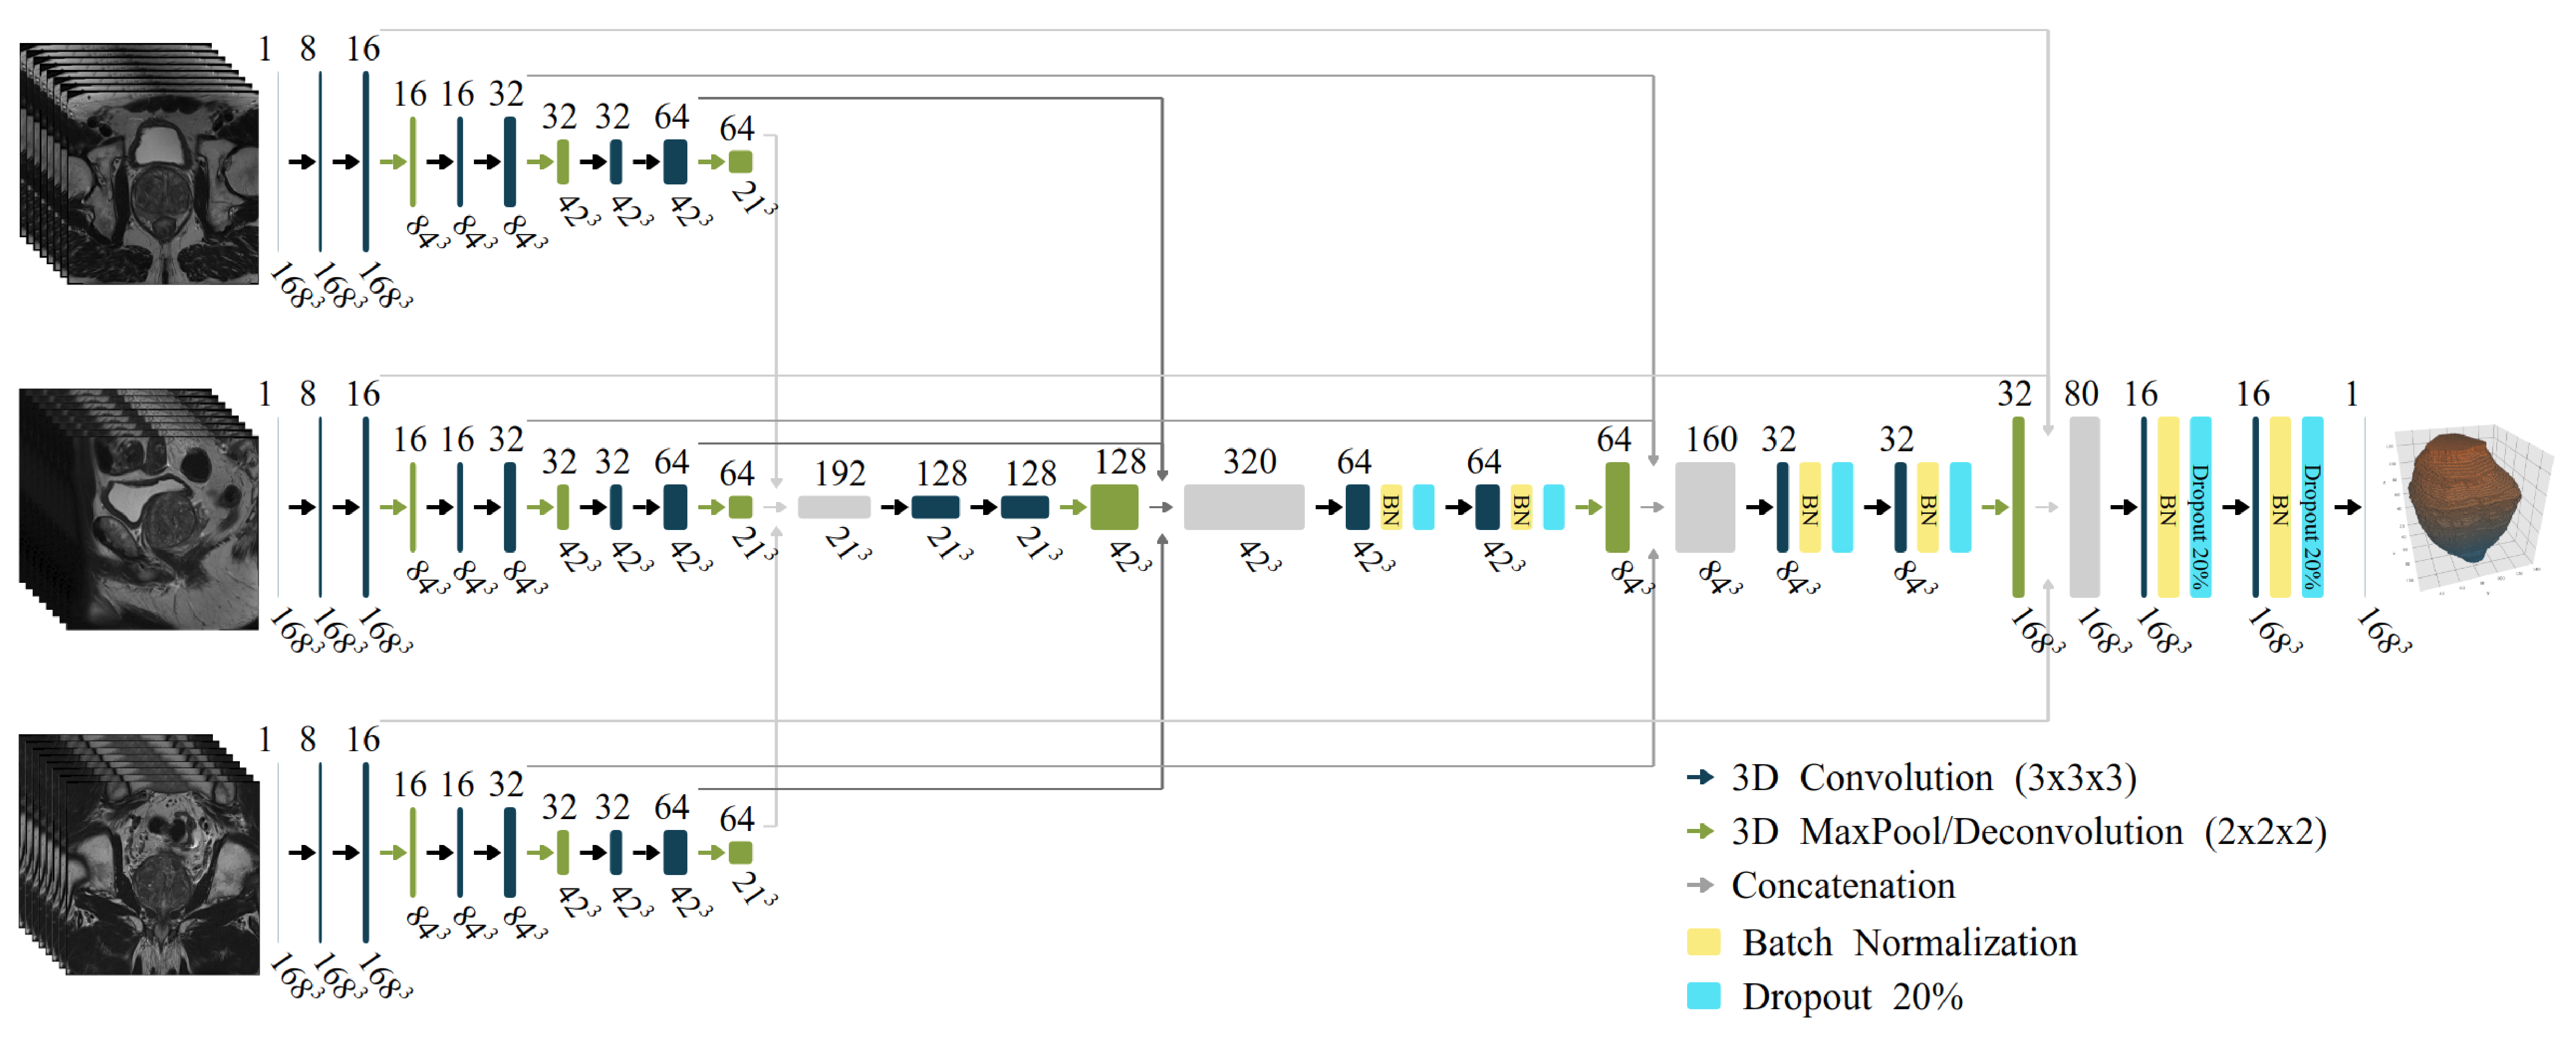
\includegraphics[totalheight=.282\textheight]{figures/Figure3.eps}
%    \caption{Multistream 3D convolutional network architecture. The input of the network are three $168^3$ volumes from the MRI planes: axial, sagittal, and coronal. }
%    \label{fig:fig_3}
%\end{figure*}
Finally, even though the CNN was trained and tested on T2-w MRIs with sizes $168^3$, the final model is not restricted to that input size and could be used with different resolutions, as long as the field of view of the isotropic input volume being used is similar to the training data. 

\subsection{Training}
\label{subsec:training}
The selected optimization algorithm is Stochastic Gradient Descent (SGD) with a learning rate $\alpha = 0.001$, momentum of 0.9 and decay of $10^{-6}$. The training is performed for 1000 epochs with an early stop mechanism if the loss function is not improved by at least $\delta = 0.001$ after 70 iterations. The Loss function used is the negative Dice Similarity Coefficient (DSC) \cite{dice1945measures}:  
\begin{equation}
\text{Loss} = - \frac{2 \sum_{i=1}^{N}p_it_i}{\sum_{i=1}^{N}p_i^2 + \sum_{i=1}^{N}t_i^2 + \varepsilon} 
\label{eq:dsc}
\end{equation}
%where N is the total number of voxels in the image, when training for prostate segmenation,
%and the number of voxels \textbf{inside} the prostate, when training for the PZ. The segmentation
%of the PZ assumes that we already know where the prostate is, so we do not take into
%account anything outside the prostate for the loss function. 
where N is the total number of voxels in the image, $p_i$ the voxel values for the prediction of the network, $t_i$ the true voxel values of the prostate or PZ masks, and $\varepsilon = 1$ for all the models.

In order to compare the robustness of the models with respect to changes in MRI vendor machines,  a distinct model was trained for each dataset: GE (n=220), Siemens (n=330), and combined model (n=550). Each dataset was split into 90\% for training and 10\% for validation. Data augmentation was performed on the fly by flipping the images in the sagittal axis and blurring them using 3D Gaussian blur randomly with $0 \leq \sigma \leq 3$. Each data augmentation method is applied with a random chance of $1/2$.  
A total number of six models are compared, three for the prostate been trained with each dataset and three more for the PZ. 

\subsection{Postprocessing}
The CNN outputs a 3D volume of the same size of the ROI, in our case $168^3$, and each voxel gets the probability of belonging to the area of interest (prostate or PZ) versus the background. From this cube, a binary mask is obtained from a threshold value of 0.5. After that, we select the largest connected volume and remove all others. Finally, we compute the 3D DSC for the contour of interest in the resampled image and in the original MRI resolution. Additionally, the prediction of the PZ contour is intersected with the prostate, restricting it to the prostate volume.

